\documentclass[11pt,a4paper,titlepage]{article}
\usepackage[brazil]{babel}
\usepackage[utf8]{inputenc}
\usepackage[T1]{fontenc}

\newcommand{\titulo}{\textit{Arquitetura de Computadores: Trabalho Prático 2 - ULA}}

\newcommand{\cabecalho}{\textit{Arquitetura de Computadores: Trabalho Prático 2 - ULA}}

\usepackage{fancyhdr}
\usepackage{indentfirst}
\usepackage{setspace}
\usepackage{graphicx,url}
%\usepackage{color,colortbl}
\usepackage{amsmath}
\usepackage{amssymb}
\usepackage{amsthm}
\usepackage{wrapfig}
\usepackage{times}
\usepackage{hyphenat}
\usepackage{ae}
\usepackage{algorithm}
\usepackage[sort,numbers]{natbib}

% Criar figura dividida em subfiguras
\usepackage{subfigure}

\usepackage{subfig}
\usepackage{ae}
\usepackage{aecompl}

\usepackage{multirow}
%\usepackage{epstopdf}

\pagestyle{fancy}

\setlength{\evensidemargin}{0.0in}
\setlength{\oddsidemargin}{0.0in}
\setlength{\textwidth}{6.6in}
\setlength{\textheight}{1.06\textheight}

\lhead{}
\chead{}
\rhead{\footnotesize{\textsc{\cabecalho}}}
\lfoot{\footnotesize{Guilherme ..., Iuri Castro, João Mateus de Freitas Veneroso, Ricardo Pagoto Marinho}}
\cfoot{}
\rfoot{\footnotesize{\thepage}}
\setlength{\headwidth}{\textwidth}
\renewcommand{\headrulewidth}{0.4pt}
\renewcommand{\footrulewidth}{0.4pt}
\renewcommand{\baselinestretch}{0.90}

%\hyphenation{ ca-rac-te-ri-zan-do--se }

\begin{document}

\begin{titlepage}
\begin{center}

\begin{large}
Universidade Federal de Minas Gerais\\
Instituto de Ciências Exatas\\
Departamento de Ciência da Computação\\
\end{large}

\vspace{20mm}

\begin{Large}
DCC007-Organização de Computadores II
\end{Large}

\vspace{20mm}

\begin{LARGE}
\titulo
\end{LARGE}


\vspace{30mm}

\begin{Large}
Guilherme ...\\ Iuri Castro\\ João Mateus de Freitas Veneroso\\ Ricardo Pagoto Marinho \\
\end{Large}


\vspace{60mm}

{\sc Belo Horizonte - MG}

{\sc \today}
%{\sc 05 de Maro de 2012}

%\vspace{10mm}
\end{center}
\end{titlepage}

%%%%%%%%%%%%%%%%%%%%%%%%%%%%%%%%%%%%%%%%%%%%%%%%%%%%%%%%%%%%%%%%%%%%%%%%%%%%%%%%%%%%%%%%%%%%%%%%%%%%%%%%%%%%%%%%%%%%%%%%%%%%%%%%%%%
%% Sumário
%\tableofcontents
%\pagebreak


%%%%%%%%%%%%%%%%%%%%%%%%%%%%%%%%%%%%%%%%%%%%%%%%%%%%%%%%%%%%%%%%%%%%%%%%%%%%%%%%%%%%%%%%%%%%%%%%%%%%%%%%%%%%%%%%%%%%%%%%%%%%%%%%%%

\section{Introdução}\label{sec-intro}

Conexões ad-hoc (sem uma infraestrutura pré-estabelecida) estão tomando cada vez mais lugar na vida das pessoas.
Através dessas conexões, usuários de dispositivos móveis podem trocar informações de maneira mais conveniente e rápida.
Além disso, já é possível jogar com outros usuários que tenham o mesmo dispositivo sem que um cabo ou uma infraestrutura de rede os conecte, apenas pareando os dispositivos.
Dessa forma, é crescente o número de possibilidades que este tipo de conexão pode entregar.

Outra ferramenta que pode ser utilizada com as conexões ad-hoc é a de roteamento, \textit{i.e.}, fazer com que dispositivos distantes um do outro possam se comunicar através de rotas criadas por outros dispositivos entre eles.
Contudo, devido a mobilidade dos dispositivos, vários tipos de protocolos de roteamento surgem como soluções para conectar os diversos dispositivos dentro da rede.

Uma das formas utilizadas é a baseada em encontros entre os dispositivos, ou seja, quando dois ou mais dispositivos estão próximos de maneira que a comunicação possa ser direta.
Durante os anos, vários protocolos de roteamento baseados em encontro foram definidos, como em~\cite{Dubois, Sarafijanovic, Grossglauser, Young-Bae}, mostrando a importância que esse tipo de roteamento possui no cenário ad-hoc.
O algoritmo proposto neste trabalho porém, incorpora informações de encontro entre dispositivos na rede para que a informação seja encaminhada.
Desta forma, apenas dispositivos com mais probabilidades de encontrar o destino receberão a informação, de modo que aumente a taxa de entrega de pacotes.

Porém, muitos protocolos acabam enviando muita informação para rede, fazendo que ela fique carregada e não consiga entregar as informações de maneira correta.
Isso acontece pois nenhuma, ou pouca, atenção é dada à quantidade de pacotes que o protocolo envia para a rede.
Uma forma de mitigar esse efeito é o algorítimo \textit{trickle timer}~\cite{Trickle}.
Com ele, é possível balancear a quantidade de informação na rede, de modo que o protocolo perceba quando é possível enviar mais pacotes e quando é necessário diminuir a quantidade de pacotes na rede, dando um balanço de informação trafegando aceitável.

Neste relatório será apresentado e definido o algoritmo de roteamento para redes ad-hoc proposto durante a disciplina de redes sem fio para o curso de Doutorado em Ciência da Computação da Universidade Federal de Minas Gerais - UFMG.

Junto com a definição do algoritmo, será apresentado também o protocolo de \textit{trickle timer} que auxilia o controle da quantidade de mensagens na rede, fazendo com que ela não fique sobrecarregada.

\subsection{Contribuições}

Aqui listo as contribuições deste trabalho:

\begin{itemize}
\item Definição de um protocolo (\textit{Encounter Path Forwarding Routing} - EPF) para encaminhamento de mensagens;
\item Mostrar que a comunicação D2D dentro da rede LTE traz benefícios à rede;
\end{itemize}

\subsection{Organização do texto}
Este projeto está organizado da seguinte forma

Os trabalhos relacionados estão listados na Seção~\ref{sec:trabRel}.
Na Seção~\ref{sec:epf} é definido e apresentado o protocolo proposto neste trabalho: EPF.
A Seção~\ref{sec:trickle} apresenta o algoritmo \textit{trickle timer} e explica seu funcionamento.
Na Seção~\ref{sec:mobPtn}, são apresentados e explicado o funcionamento dos padrões de mobilidade utilizados no trabalho.
Já a Seção~\ref{sec:imp}, explica como o algorítimo EPF foi implementado e testado, enquanto a Seção~\ref{sec:limit} mostra algumas das limitações encontradas para o algorítimo.
A Seção~\ref{sec:conf} mostra as configurações utilizadas nos testes para a obtenção dos resultados.
Na Seção~\ref{sec:results} os resultados são apresentados e discutidos.
Por último, a Seção~\ref{sec-consideracoes}, traz as considerações finais.

\section{Trabalhos relacionados}\label{sec:trabRel}

Em~\cite{Spyropoulos}, os autores propões o protocolo \textit{Spray-and-Wait}, baseado no protocolo de \textit{flooding}, os seja, disseminação de informações.
Contudo, diferentemente do \textit{flooding}, o protocolo proposto pelos autores não envia várias vezes as informações assim que encontrar outros nós da rede.
Um nó que deseja se comunicar envia uma quantidade de cópias da para os nós e espera até que um deles encontre o destino.
Com isso, ele garante que menos informações serão inseridas na rede, já que apenas o nó que inicia a comunicação faz o \textit{Spray}.
Porém, não há garantias que algum nó encontrará o destino, apesar de ser pouco provável esse caso.

Os autores de~\cite{Crowcroft} propõem o algoritmo \textit{BUBBLE Rap}.
Este algoritmo utiliza duas informações para encaminhar as mensagens: i) localização do destino e ii) centralidade dos nós na localização.
Primeiro, todos os nós na rede são rotulados de acordo com sua localização.
Então, quando um nó deseja se comunicar com outro, ele deve informar a qual rótulo o destino pertence.
Dessa forma, a mensagem sempre é encaminhada para um nó que esteja em uma localização mais próxima da do destino.
Quando a mensagem chega em um nó que esteja com o mesmo rótulo, portanto, perto do destino, a mensagem é enviada para o nó mais central.
Ele, por sua vez, fica responsável por entregar a mensagem ao destino.

\cite{Xiao} fazem o roteamento de dispositivos em IMSN - \textit{Impromptu Mobile Social Networks}~(\cite{Xiao}).
Os dispositivos na rede armazenam informações sobre outros nos quais já tiveram contato anteriormente e as utilizam para decidir para quem enviar a mensagem.
Além de informação sobre contato, como a quantidade de vezes que dois dispositivos se encontram em um intervalo de tempo, os algoritmos propostos utilizam informações sociais, como localização atual, local de estudo e/ou trabalho entre outros, para tentarem predizer para qual dispositivo encaminhar a mensagem.
Essas informações são referentes ao destino, de forma que um dispositivo só encaminhará a mensagem para um outro que seja mais relacionado com o destino, aumentando as chances de entrega da mensagem.

Além disso, as métricas sociais são balanceadas pela quantidade de vezes que um determinado dispositivo encontrou outro que possua aquela métrica, \textit{e.g.}, se as métricas "Mora em Belo Horizonte"~e "Frequenta a UFMG"~forem utilizadas, um dispositivo \textit{x} pode se encontrar mais vezes com outro \textit{y} que "Mora em Belo Horizonte"~do que com outro \textit{z} que "Frequenta a UFMG".
Logo, se o destino \textit{d} também possui a métrica "Mora em Belo Horizonte", \textit{x} terá maior probabilidade de enviar a mensagem para \textit{y} do que para \textit{z}.

Com base nessas duas métricas, foram criados dois algoritmos: \textit{Hisso} e \textit{Enhanced Hisso}.
Eles utilizam cálculos diferentes para definir o valor de cada métrica.
Além disso, eles fazem o roteamento de acordo com um peso dado a cada uma das métricas, sendo uma mais importante que a outra na hora de definir o próximo dispositivo a receber a mensagem.

Já em~\cite{Lindgren}, o protocolo \textit{PROPHET} é proposto.
Nele, os autores utilizam uma métrica probabilística para determinar se um nó receberá ou não a mensagem para o destino.
Cada nó tem uma métrica associada aos outros nós da rede e, baseados nela, eles saberão se podem ou não encaminhar a mensagem.
Essa decisão é tomada no caso de um nó ter uma probabilidade maior de encontrar com o destino do que o nó atual que tem a mensagem.
Além disso, sempre que os nós se encontram, as informações 
 de probabilidade de encontro são trocadas para que estejam sempre atualizadas.
\section{EPF}
\label{sec:epf}

O algorítimo EPF se baseia em encaminhamento das mensagens através de encontros entre os dispositivos.
Desta forma, se um dispositivo \textit{a} que deseja se comunicar com um outro dispositivo \textit{c} encontra um \textit{b}, a mensagem de \textit{a} para \textit{c} pode ser transmitida por \textit{b}.

Para que a transmissão ocorra, algumas regras devem ser seguidas.
Durante todo o tempo, os dispositivos vão guardando com quais outros eles se encontraram, para que eles possam escolher de maneira mais eficiente, qual irá receber a mensagem que chegará ao destino.

Para a decisão, toda vez que os dispositivos se encontram, eles armazenam a quantidade de tempo que o contato ocorreu.
Assim, quanto mais vezes e por mais tempo dois dispositivos se encontrarem, maior esse número.
A informação é passada do dispositivo \textit{a} para o dispositivo \textit{b} com destino a \textit{c} se:
\begin{itemize}
\item o tempo de contato for maior do que um limiar pré-estabelecido;
\item o tempo de contato entre \textit{b} e \textit{c} for maior do que o tempo de contato entre \textit{a} e \textit{c};
\item o tempo de contato entre \textit{b} e \textit{c} for maior do que o limiar pré-estabelecido.
\end{itemize}

Apenas no caso em que os três requisitos sejam alcançado a informação é encaminhada.
Quando o dispositivo \textit{b} encontrar \textit{c}, ele encaminha a mensagem diretamente sem que haja nenhum tipo de condição.

As Figuras~\ref{fig:ok1},~\ref{fig:nok1} e~\ref{fig:nok2} exemplificam essas decisões.

\begin{figure}
\centering
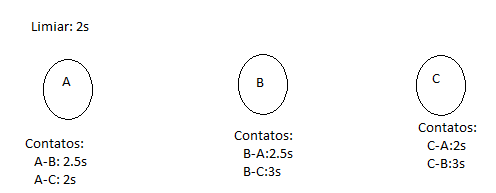
\includegraphics[]{images/ok1.png}
\caption{Transmissão ok.}
\label{fig:ok1}
\end{figure}

Na Figura~\ref{fig:ok1}, a transmissão ocorre pois todos os requisitos são respeitados, \textit{i.e.}, o contato entre \textit{a} e \textit{a} é maior do que o limiar (2s nesse caso), o contato entre \textit{a} e \textit{a} é maior do que o contato entre \textit{a} e \textit{c} e o contato entre \textit{b} e \textit{c} é maior do que o limiar

\begin{figure}
\centering
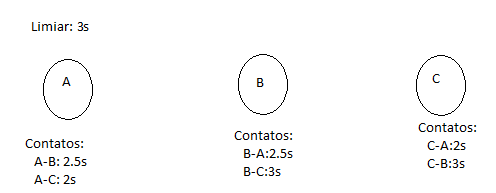
\includegraphics[]{images/nok1.png}
\caption{Contatos menores do que limiar.}
\label{fig:nok1}
\end{figure}

Já na Figura~\ref{fig:nok1}, a transmissão não ocorre, pois nenhum contato entre os dispositivos é maior do que o limiar (3s).
Dessa forma, por hora, não existem transmissões na rede.

\begin{figure}[h]
\centering
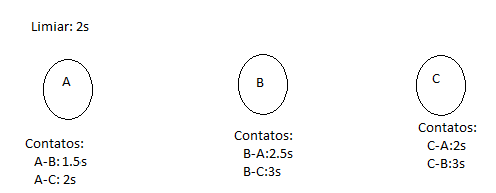
\includegraphics[]{images/nok2.png}
\caption{Contato entre A e B menor do que limiar.}
\label{fig:nok2}
\end{figure}

A Figura~\ref{fig:nok2} mostra outra situação onde a transmissão não ocorre.
Apesar de o contato entre \textit{b} e \textit{c} obedecerem as regras, ou seja, ser maior do que o contato entre \textit{a} e \textit{c} e maior do que o limiar (2s), o contato entre \textit{a} e \textit{b} é menor do que o limiar.
Assim, \textit{a} considera \textit{b} como não sendo um bom dispositivo para receber a mensagem, já que eles não tem muito tempo de contato.

Desta forma, o algorítimo favorece dispositivos que possuem mais tempo de contatos, pois considera esses dispositivos mais seguros no encaminhamento da mensagem até o destino.

\section{\textit{Trickle timer}}\label{sec:trickle}

O algorítimo \textit{trickle timer} faz com que, ao invés de os nós inundarem a rede com pacotes, eles escutem a rede para que um número máximo de pacotes esteja presente na rede, de forma que ela fique consistente.
Originalmente, este algorítimo foi desenvolvido para reprogramar protocolos, \textit{i.e.}, o dado enviado por ele é a parte do protocolo que deve ser atualizado.
Porém, ele se mostrou mais robusto e pôde ser utilizado em diversas situações, como, controle de tráfego, de propagação \textit{multicast}, roteamento, etc.

A base do algorítimo são as decisões dos nós na rede sobre a consistência da informação recebida.
Essa consistência pode ser baseada em número de sequência de pacotes esperado pelo nó.
Dessa forma, um nó diz que a informação está consistente se o número de sequência para aquele pacote é o esperado, e diz que não está consistente se recebe um número diferente do esperado.
Por exemplo, se o nó \textit{A} envia um pacote com um número \textit{N} para \textit{B}, mas este está esperando \textit{N+1}, \textit{B} sabe que \textit{A} está desatualizado.
Da mesma forma, se \textit{B} envia \textit{N+1} para \textit{A}, e \textit{A} possui \textit{N}, \textit{A} perceberá que está desatualizado.

O algorítimo possui alguns parâmetros e variáveis.
Os primeiros são os limites de intervalos de comunicação (em ms): $I_{min}$ como limite inferior e $I_{max}$ como limite superior, sendo que $I_{max}$ é o dobro de $I_{min}$.
Além desses dois parâmetros, o algorítimo possui um número inteiro maior que zero \textit{k}, indicando o número máximo de mensagens na rede.

Três variáveis são mantidas pelo algorítimo: \textit{I}, \textit{t} e \textit{c}.
\textit{I} é o intervalo de tempo de comunicação colocado no intervalo [$I_{min}$,$I_{max}$], \textit{t} é um tempo dentro do intervalo \textit{I}, colocado entre [\textit{$\frac{I}{2}$,I)} e \textit{c} é um contador de mensagens na rede.
Quando o algorítimo inicia, o valor de \textit{I} é definido e somente nesse intervalo de tempo ele executa.
Sempre que um intervalo inicia, o valor de \textit{c} é colocado em 0 e o valor de \textit{t} é definido.
Os nós enviam as mensagem no tempo \textit{t} e caso o valor de \textit{c} seja menor do que \textit{k}.
Quando um nó recebe uma mensagem consistente, ele incrementa o valor de \textit{c}.
No fim do intervalo \textit{I}, o algorítimo dobra este valor até o máximo de $I_{max}$.
Por fim, quando uma mensagem recebida é inconsistente e \textit{I} é maior do que $I_{min}$, o algorítimo é reiniciado.
Para isso, \textit{I} é definido como sendo o valor de $I_{min}$ e \textit{t} é definido novamente da mesma forma do início do algorítimo (colocado entre [\textit{$\frac{I}{2}$,I)}).
Caso \textit{I} for igual a $I_{min}$ na detecção da inconsistência, nada acontece.

%%%%%%%%%%%%%%%%%%%%%%%%%%%%%%%%%%%%%%%%%%%%%%%%%%%%%%%%%%%%%%%%%%%%%%%%%%%%%%%%%%%%%%%%%%%%%%%%%%%%%%%%%%%%%%%%%%%%%%%%%%%%%%%%%%%

\section{Padrões de mobilidade}
\label{sec:mobPtn}

Os dispositivos são, geralmente, carregados por pessoas.
As pessoas, por sua vez, se movimentam constantemente durante o dia, seja se movendo de casa para o trabalho, para o local de estudo ou para fazer alguma outra coisa.
Em um primeiro momento, podemos pensar que as pessoas se movimentam aleatoriamente, ou seja, sem nenhum padrão definido.
Segundo~\cite{Jie}, padrão de mobilidade é a movimentação regular de pessoas no espaço-tempo.
Além disso, eles dizem que existem dois tipos de mobilidade: i) individual e ii) global.
O primeiro se refere ao indivíduo apenas, já o segundo se refere à movimentação de uma massa de indivíduos, podendo ser utilizada em planejamento urbano.

As redes ad-hoc móveis - \textit{Mobile ad-hoc Networks} (MANETs) - possuem a característica de serem móveis.
Os nós que fazem parte dela podem se mover livremente dentro da rede, trazendo outros desfios.
Desta forma, utilizamos o \textit{Random Waypoint} - RWP~(\cite{RWP}), \textit{Reference Point Group Model} -RPGM~(\cite{RPGM}) - e RWP+RPGM.
O RWP distribui aleatoriamente pontos dentro de um espaço e cria caminhos entre eles.
Os nós são distribuídos aleatoriamente entre esses pontos e escolhem, também de modo aleatório, um outro ponto para chegar.
Assim que o nó chega no ponto destino, ele espera um tempo aleatório antes de escolher outro ponto para se mover novamente.

O RPGM simula movimentação de grupos.
Nele um dos nós é o "guia", ou seja, ele que vai dizer para aonde o grupo irá.
Primeiro o nó "guia", que aqui chamamos de nó central, é colocado em um ponto e é determinado um outro ponto destino para ele.
Os outros nós são colocados aleatoriamente em volta do nó central.
Para ir de um ponto a outro, são definidos \textit{checkpoints} para o nó central, ao chegar em um \textit{checkpoint}, ele calcula a direção para chegar ao próximo.
Assim que chegar, outro ponto de destino é definido e a movimentação é retomada.

Este padrão pode ser encarado como um guia turístico.
O guia leva um grupo através de vários pontos até chegar a um último que é o final.

O último tipo de padrão de mobilidade é uma combinação dos dois anteriores.
Nele, metade dos nós se movimentam seguindo o padrão RWP e a outra metade seguindo o padrão RPGM.
Essa decisão foi tomada para verificar como os protocolos se comportam em cenários com diferentes padrões de mobilidade.

\section{Implementação}\label{sec:imp}

Aqui será discutido detalhes da implementação do algorítimo EPF.
O ambiente utilizado foi o simulador de eventos Omnet++ 5.0 com Windows 10.

Para que a transmissão dos dados ocorresse, algumas mensagens foram criadas:

\begin{itemize}
\item \textit{Contact Info}
\item \textit{Require Message}
\item \textit{Response Message}
\end{itemize}

A primeira mensagem (\textit{Contact Info}) serve para que os nós armazenem as informações de contatos com seus vizinhos.
Assim, sempre que um nó recebe esta mensagem, ele incrementa o tempo de contato (com base no último contato recebido) caso já tenha existido um contato ou cria uma entrada na tabela de contatos para o novo dispositivo caso nenhum contato anterior ocorreu.

Já a mensagem \textit{Require Message} funciona como um pedido de autorização de envio do dado.
No exemplo anterior dos dispositivos \textit{a},\textit{b} e \textit{c}, quando \textit{a} encontra \textit{b}, ele envia uma dessas mensagens para saber se \textit{b} pode receber o dado.
Assim que recebe-lá, \textit{b} faz as verificações descritas na seção~\ref{sec:epf} para saber se pode ou não receber a mensagem.

Já a mensagem \textit{Response Message} é a resposta do dispositivo informando se pode ou não receber a mensagem.
Se as verificações em \textit{b} estiverem corretas, ele envia a \textit{a} uma mensagem de resposta \textit{ok}, informando que pode receber o dado.
Se, por outro lado, alguma verificação estiver incorreta, \textit{b} envia a \textit{a} uma mensagem de resposta \textit{not ok}, informando que não pode receber o dado.
No caso de uma negativa de \textit{b}, \textit{a} não sabe o real motivo dela, apenas que \textit{b} não pode receber a informação.

\section{Limitações}\label{sec:limit}

Diante da implementação do protocolo EPF, algumas limitações foram detectadas.
Uma delas é que o tempo de contato entre os dispositivos não é reiniciado, fazendo que, após um tempo razoavelmente grande, todos os dispositivos poderão receber as mensagens.
Contudo, essa configuração pode ocorrer em um cenário no qual o dispositivo que recebe a mensagem para encaminhamento não esteja mais perto do destino ou de outro candidato melhor.
Isso pode ocorrer pois a informação de contato pode ser antiga, da forma que no começo da simulação, os dispositivos estavam perto, mas no momento do encaminhamento, eles não estão mais.

Outra limitação é que quem decide se a mensagem pode ou não ser encaminhada é o dispositivo que irá recebe-lá, fazendo que dispositivos maliciosos ajam livremente.
Um dispositivo pode dizer que pode receber a mensagem, mas na verdade não é indicado para tal, fazendo que a mensagem se perca na rede ou pode dizer que ele não pode receber a mensagem, mesmo sendo um dispositivo indicado, fazendo que a mensagem demore ou nunca chegue ao destino.

\begin{figure}[ht]
\centering
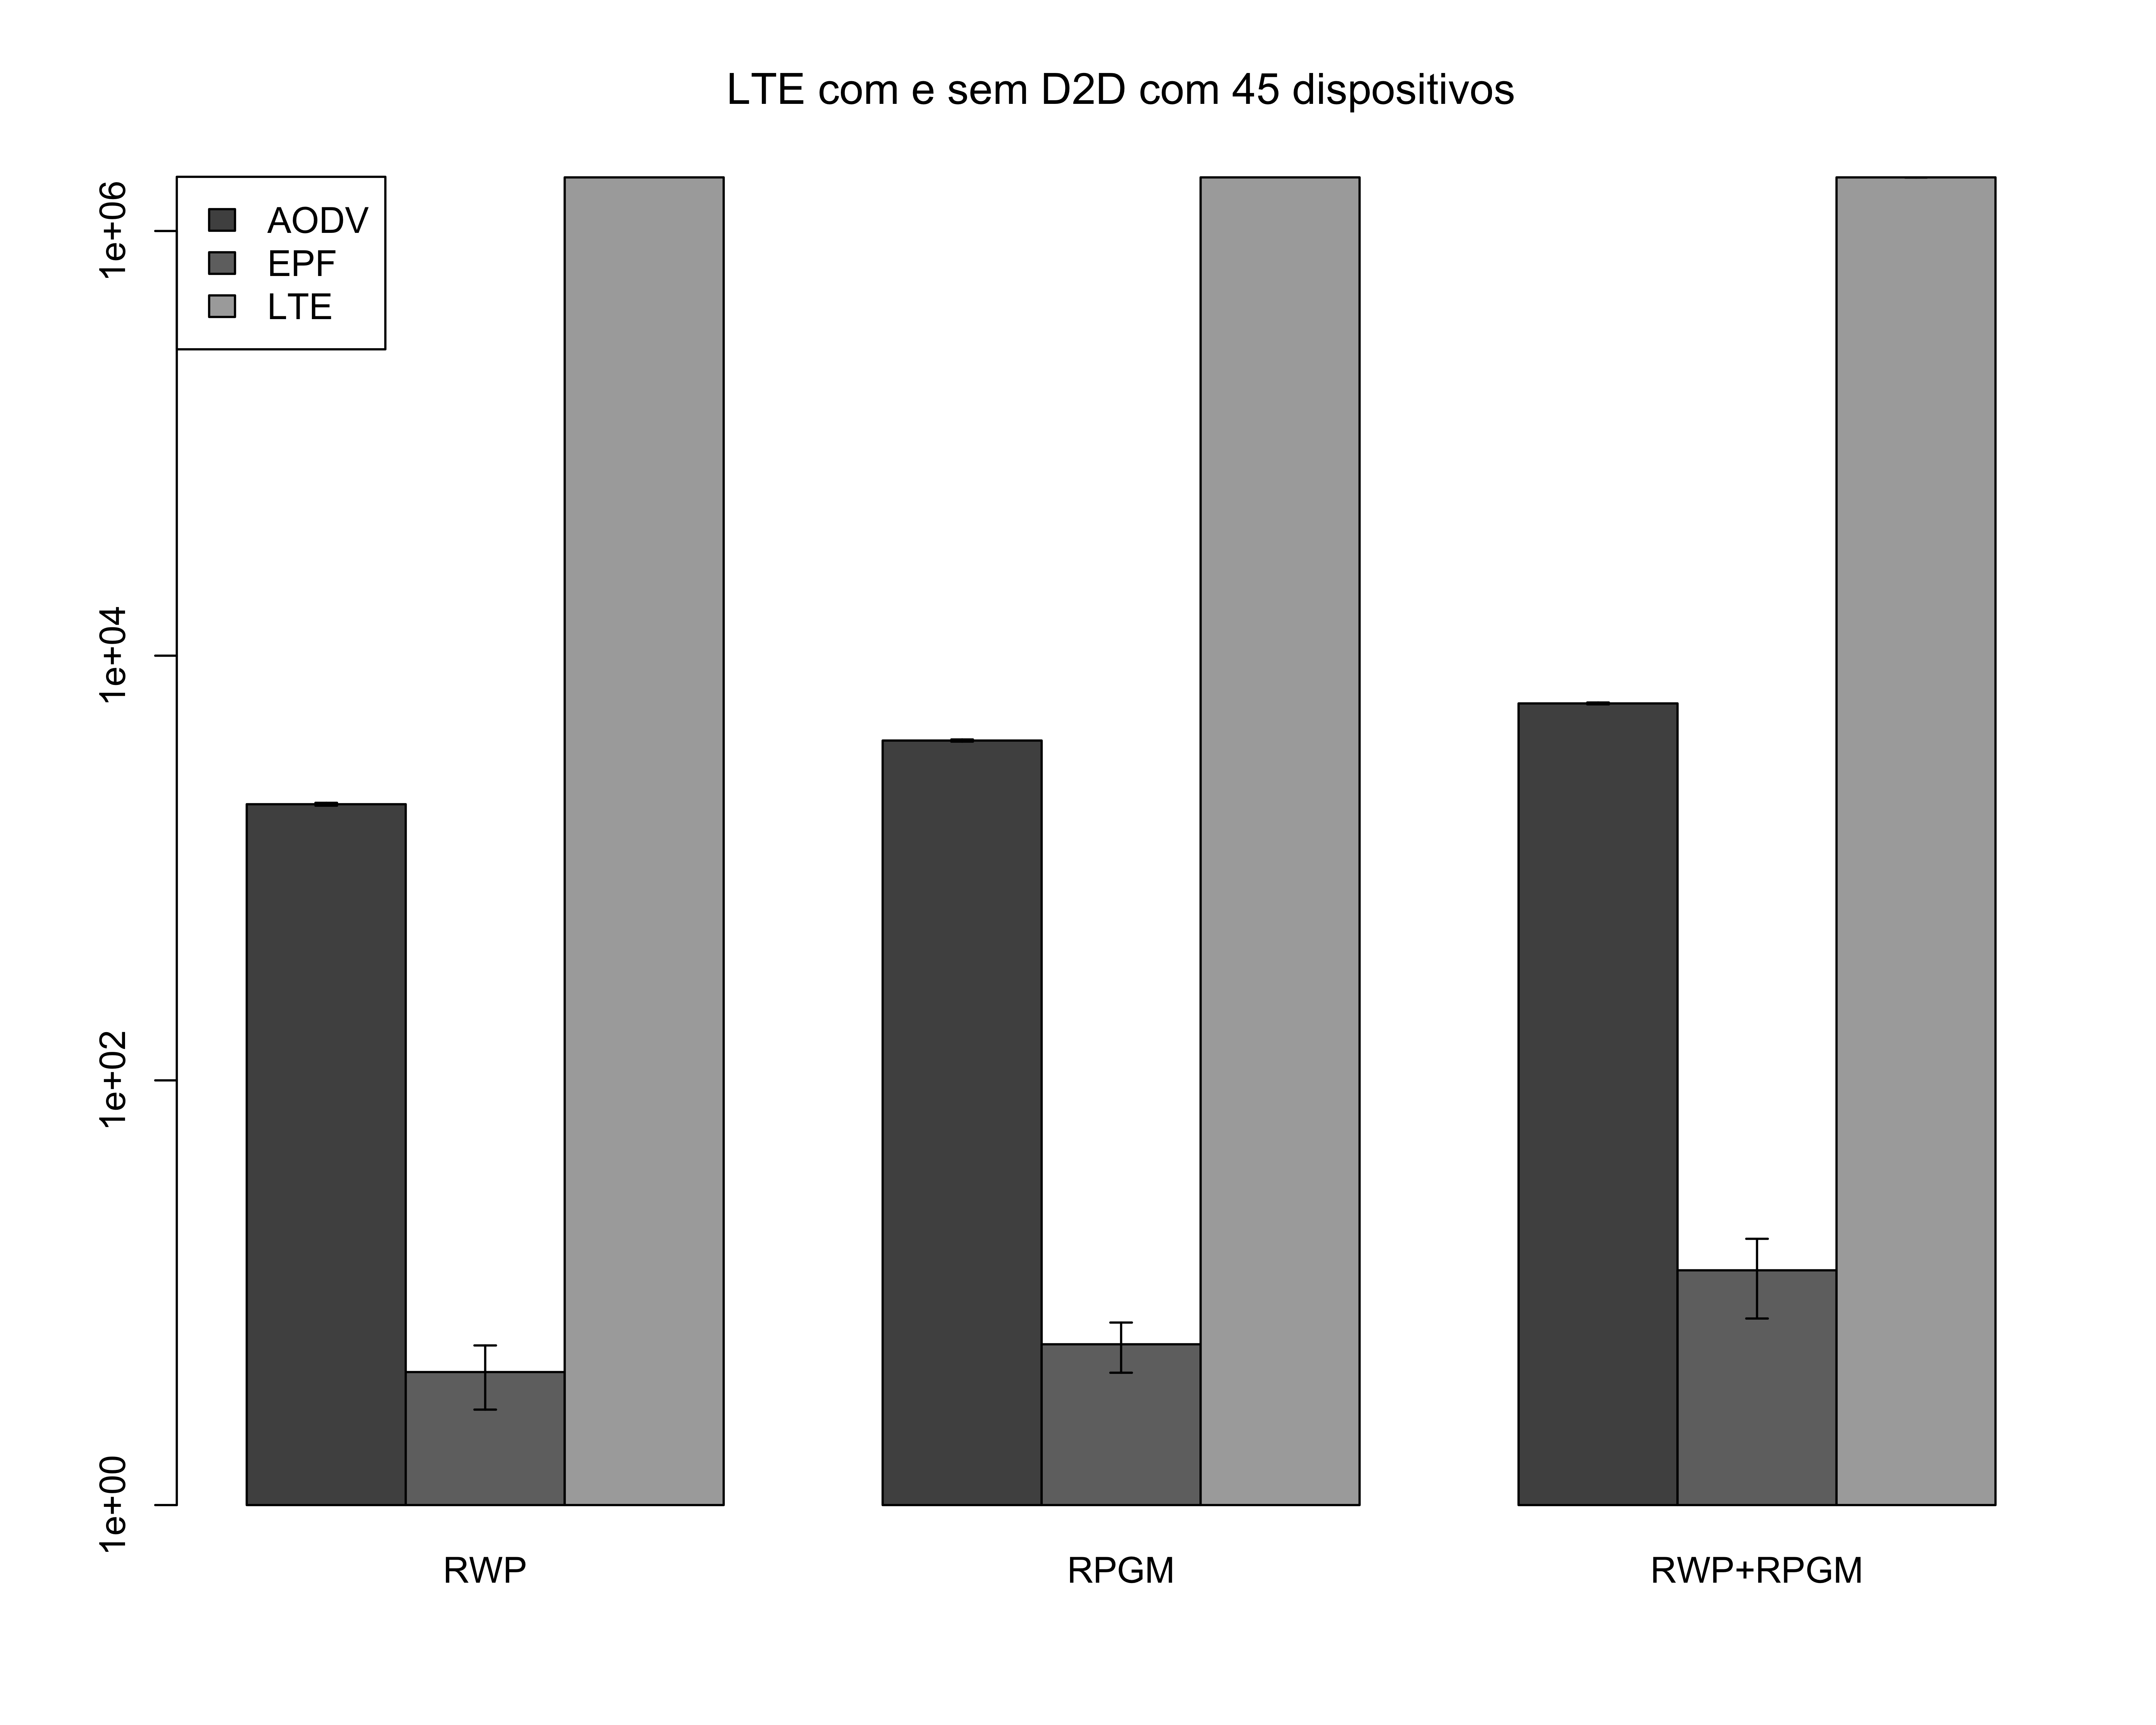
\includegraphics[height=8cm, width=0.9\textwidth]{images/complte.jpg}
\caption{Comparação entre LTE e LTE com D2D.}
\label{fig:lte}
\end{figure}

\section{Configurações}\label{sec:conf}

Agora será discutidas as configurações dos cenários utilizados nos testes.

Primeiro, comparei a carga na rede LTE normal, sem D2D, com a rede LTE utilizando D2D para saber qual o ganho real quando introduzimos a comunicação entre os dispositivos na rede com um intervalo de confiança de 99\% .
Nessa comparação, os nós não se movimentavam, apenas faziam a comunicação com a BS (LTE) e com os demais dispositivos (D2D).
Feito isso, utilizando a configuração de comunicação D2D na rede LTE, dois protocolos foram utilizados: i)AODV e ii)EPF.
Essa comparação visa mostrar se o protocolo proposto se sai melhor, em termos de quantidade de mensagens entregue ao destino, porcentagem de mensagens perdidas, tempo de enfileiramento nos \textit{buffers} e porcentagem da quantidade de mensagens que chegam fora de ordem do que um clássico.
Por fim, utilizamos o algoritmo de \textit{trickle} para ver as mudanças que ele traz ao EPF.
Nas comparações dos protocolos, o intervalo de confiança utilizado foi de 90\%.

Para o \textit{trickle} as configurações foram:

\begin{itemize}
\item $I_{min}$: 10s
\item $I_{max}$: 20s
\item \textit{k}: 5 mensagens
\end{itemize}

Os valores de $I_{min}$ e $I_{max}$ foram escolhidos arbitrariamente, enquanto o de \textit{k} foi escolhido com base na especificação do algoritmo em seu site(~\cite{Trickle}).

\begin{figure}[ht]
\centering
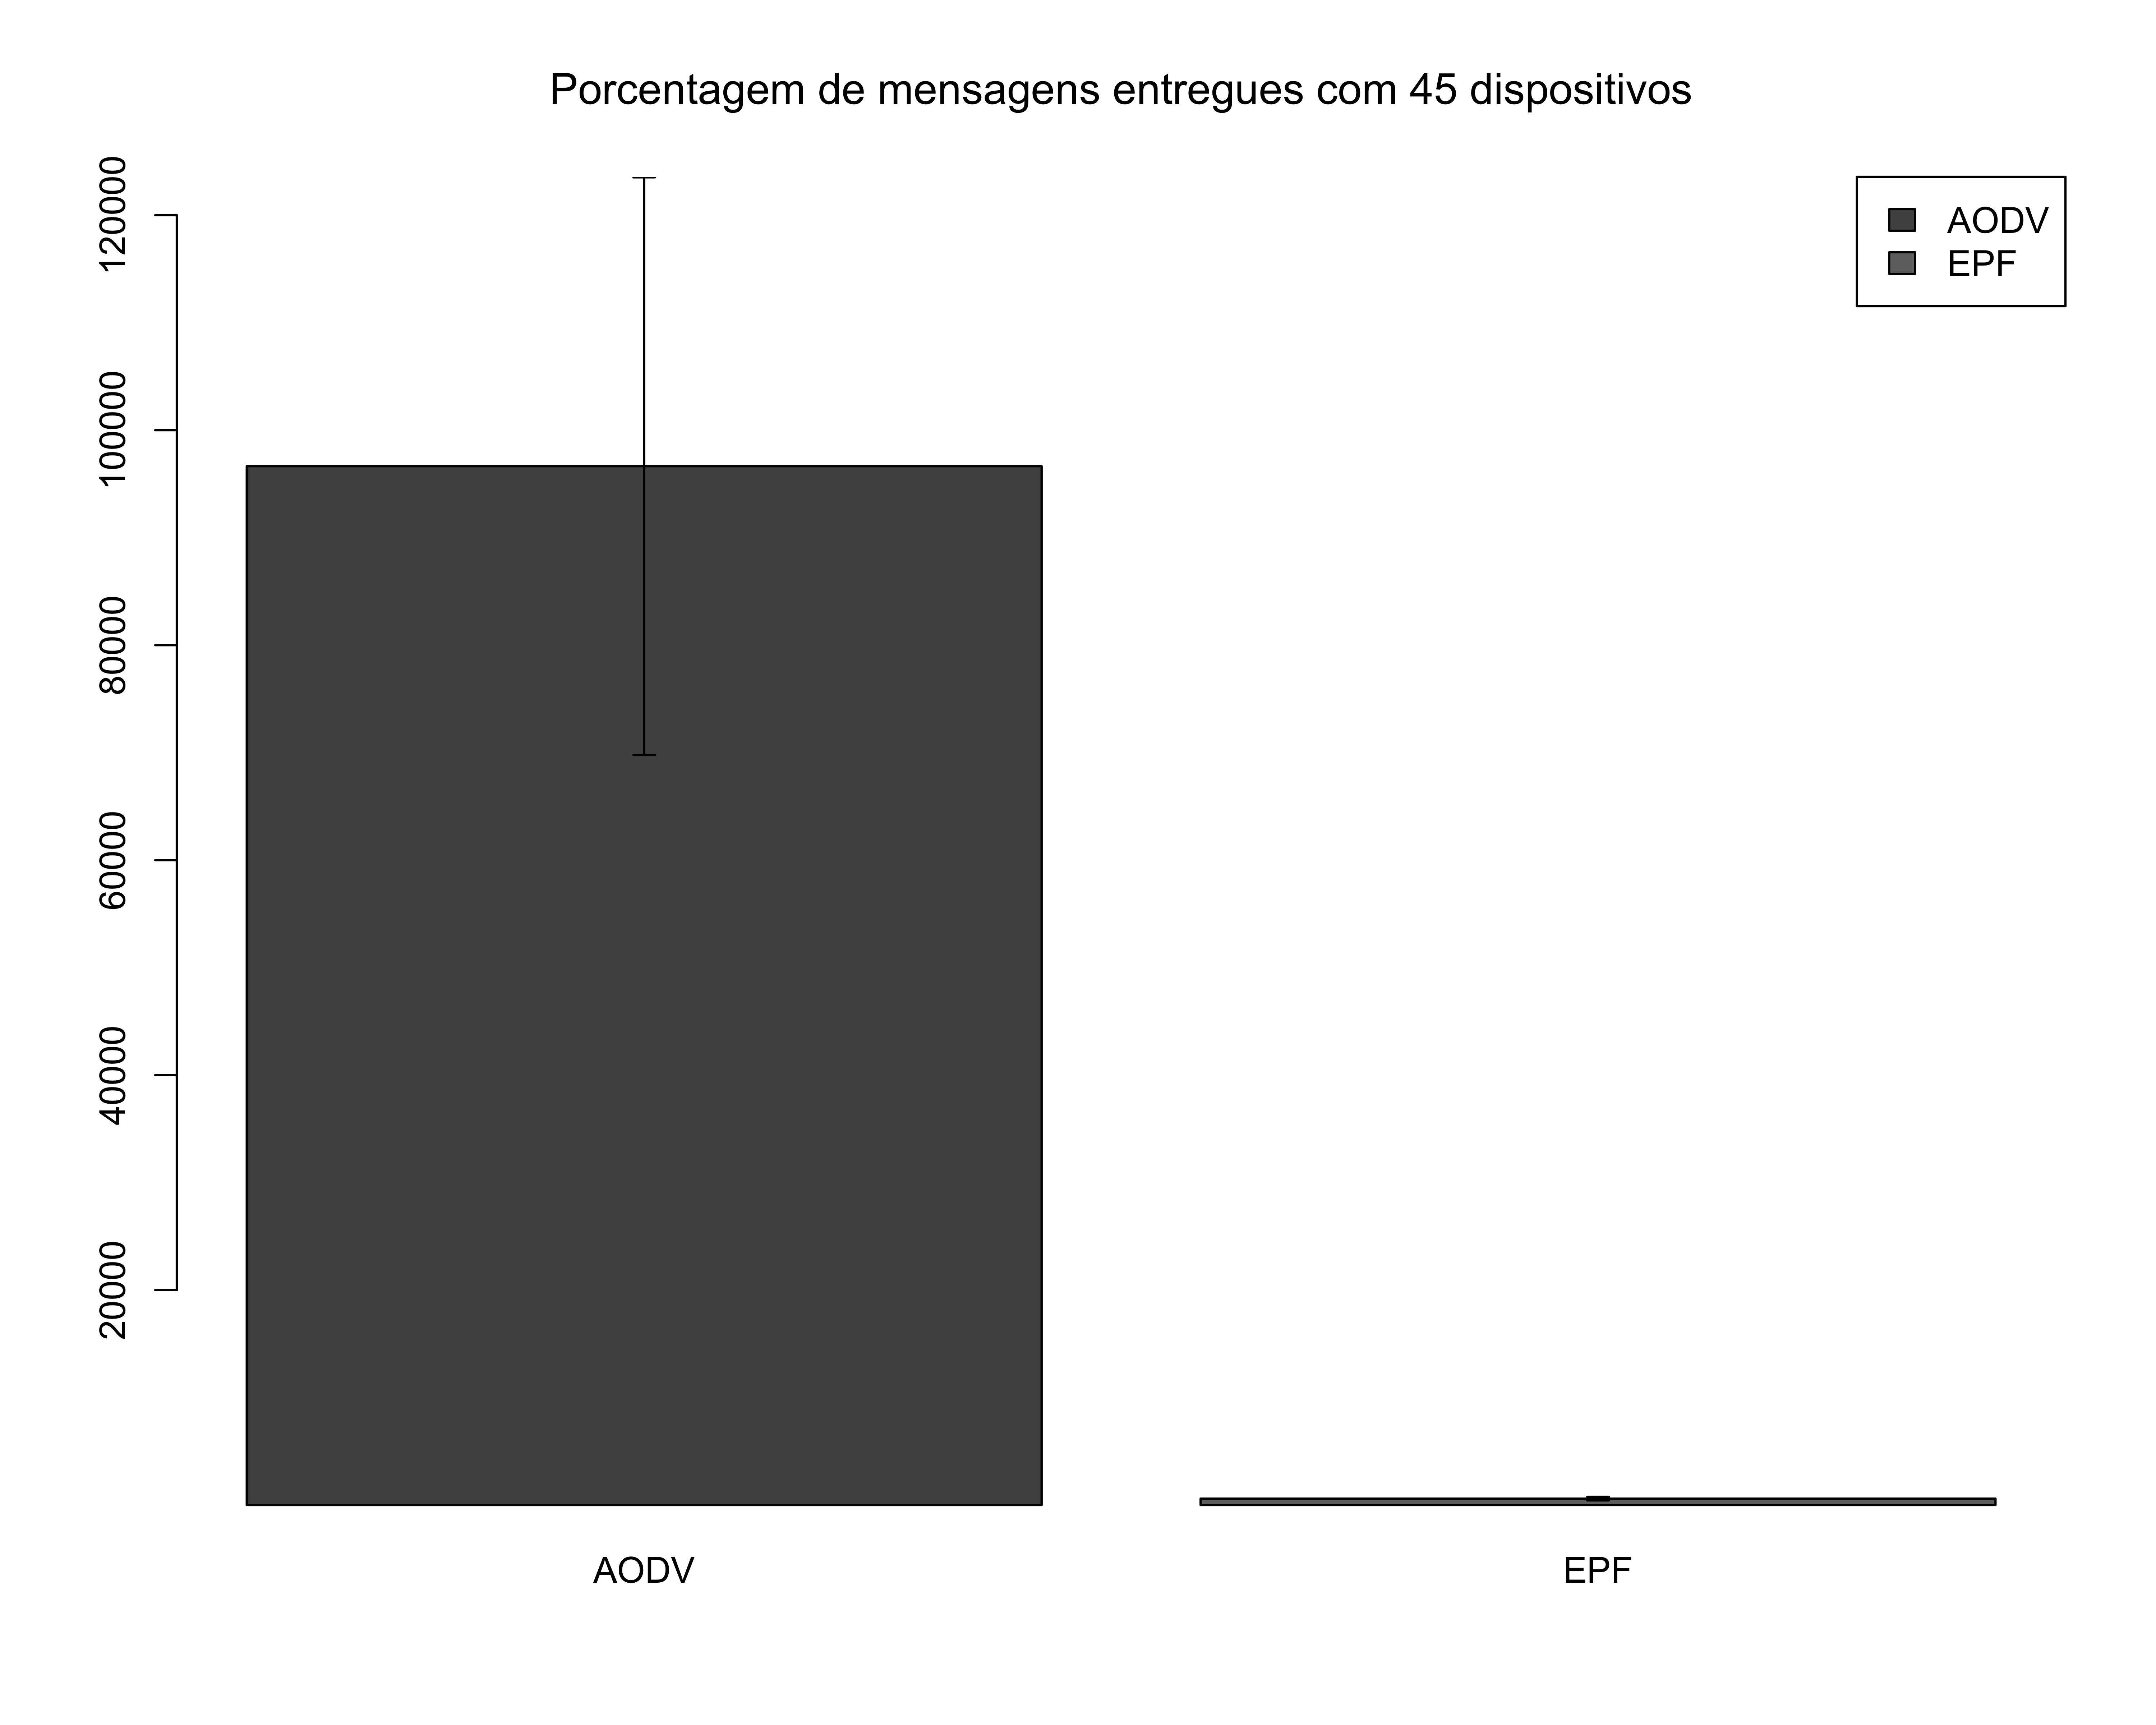
\includegraphics[height=8cm, width=0.9\textwidth]{images/entr.jpg}
\caption{Média de mensagens entregues.}
\label{fig:entr}
\end{figure}


No cenário com D2D, a torre escolhe aleatoriamente um nó e indica, também aleatoriamente, outro nó para que ele faça a comunicação.
Para os cenários LTE e LTE+D2D foram utilizadas as configurações definidas pelo Omnet++:
%\captionsetup{font={footnotesize,sc},justification=centering,labelsep=period}%
\begin{table}[t]
\caption{Configuração Cenário LTE}
\centering
\begin{tabular}{| l | l |}
\hline
Parâmetro & Valor\\
\hline
Número de nós & 45 \\
\hline
Frequência & 2 GHz \\
\hline
Altura da BS & 25m \\
\hline
Altura do prédio & 20m \\
\hline
Atenuação do sinal & Habilitado\\
\hline
Tipo de atenuação & JAKES\\
\hline
Área & 600 m x 600 m\\
\hline
\end{tabular}
\label{tab:lte-param}
\end{table}

Em todos os testes, foram utilizados 30 e 45 dispositivos na rede repetindo 35 vezes cada configuração.
Além disso, no cenário com D2D foram utilizados três padrões de mobilidade: i)\textit{Random Waypoint} (RWP), ii)\textit{Reference Point Group Model} (RPGM) e iii) RWP+RPGM onde metade dos dispositivos se movimentavam com um padrão e a outra metade com outro.
Em todos os padrões, os nós se movimentavam com uma velocidade de 0.5 m/s.

\begin{figure}[ht]
\centering
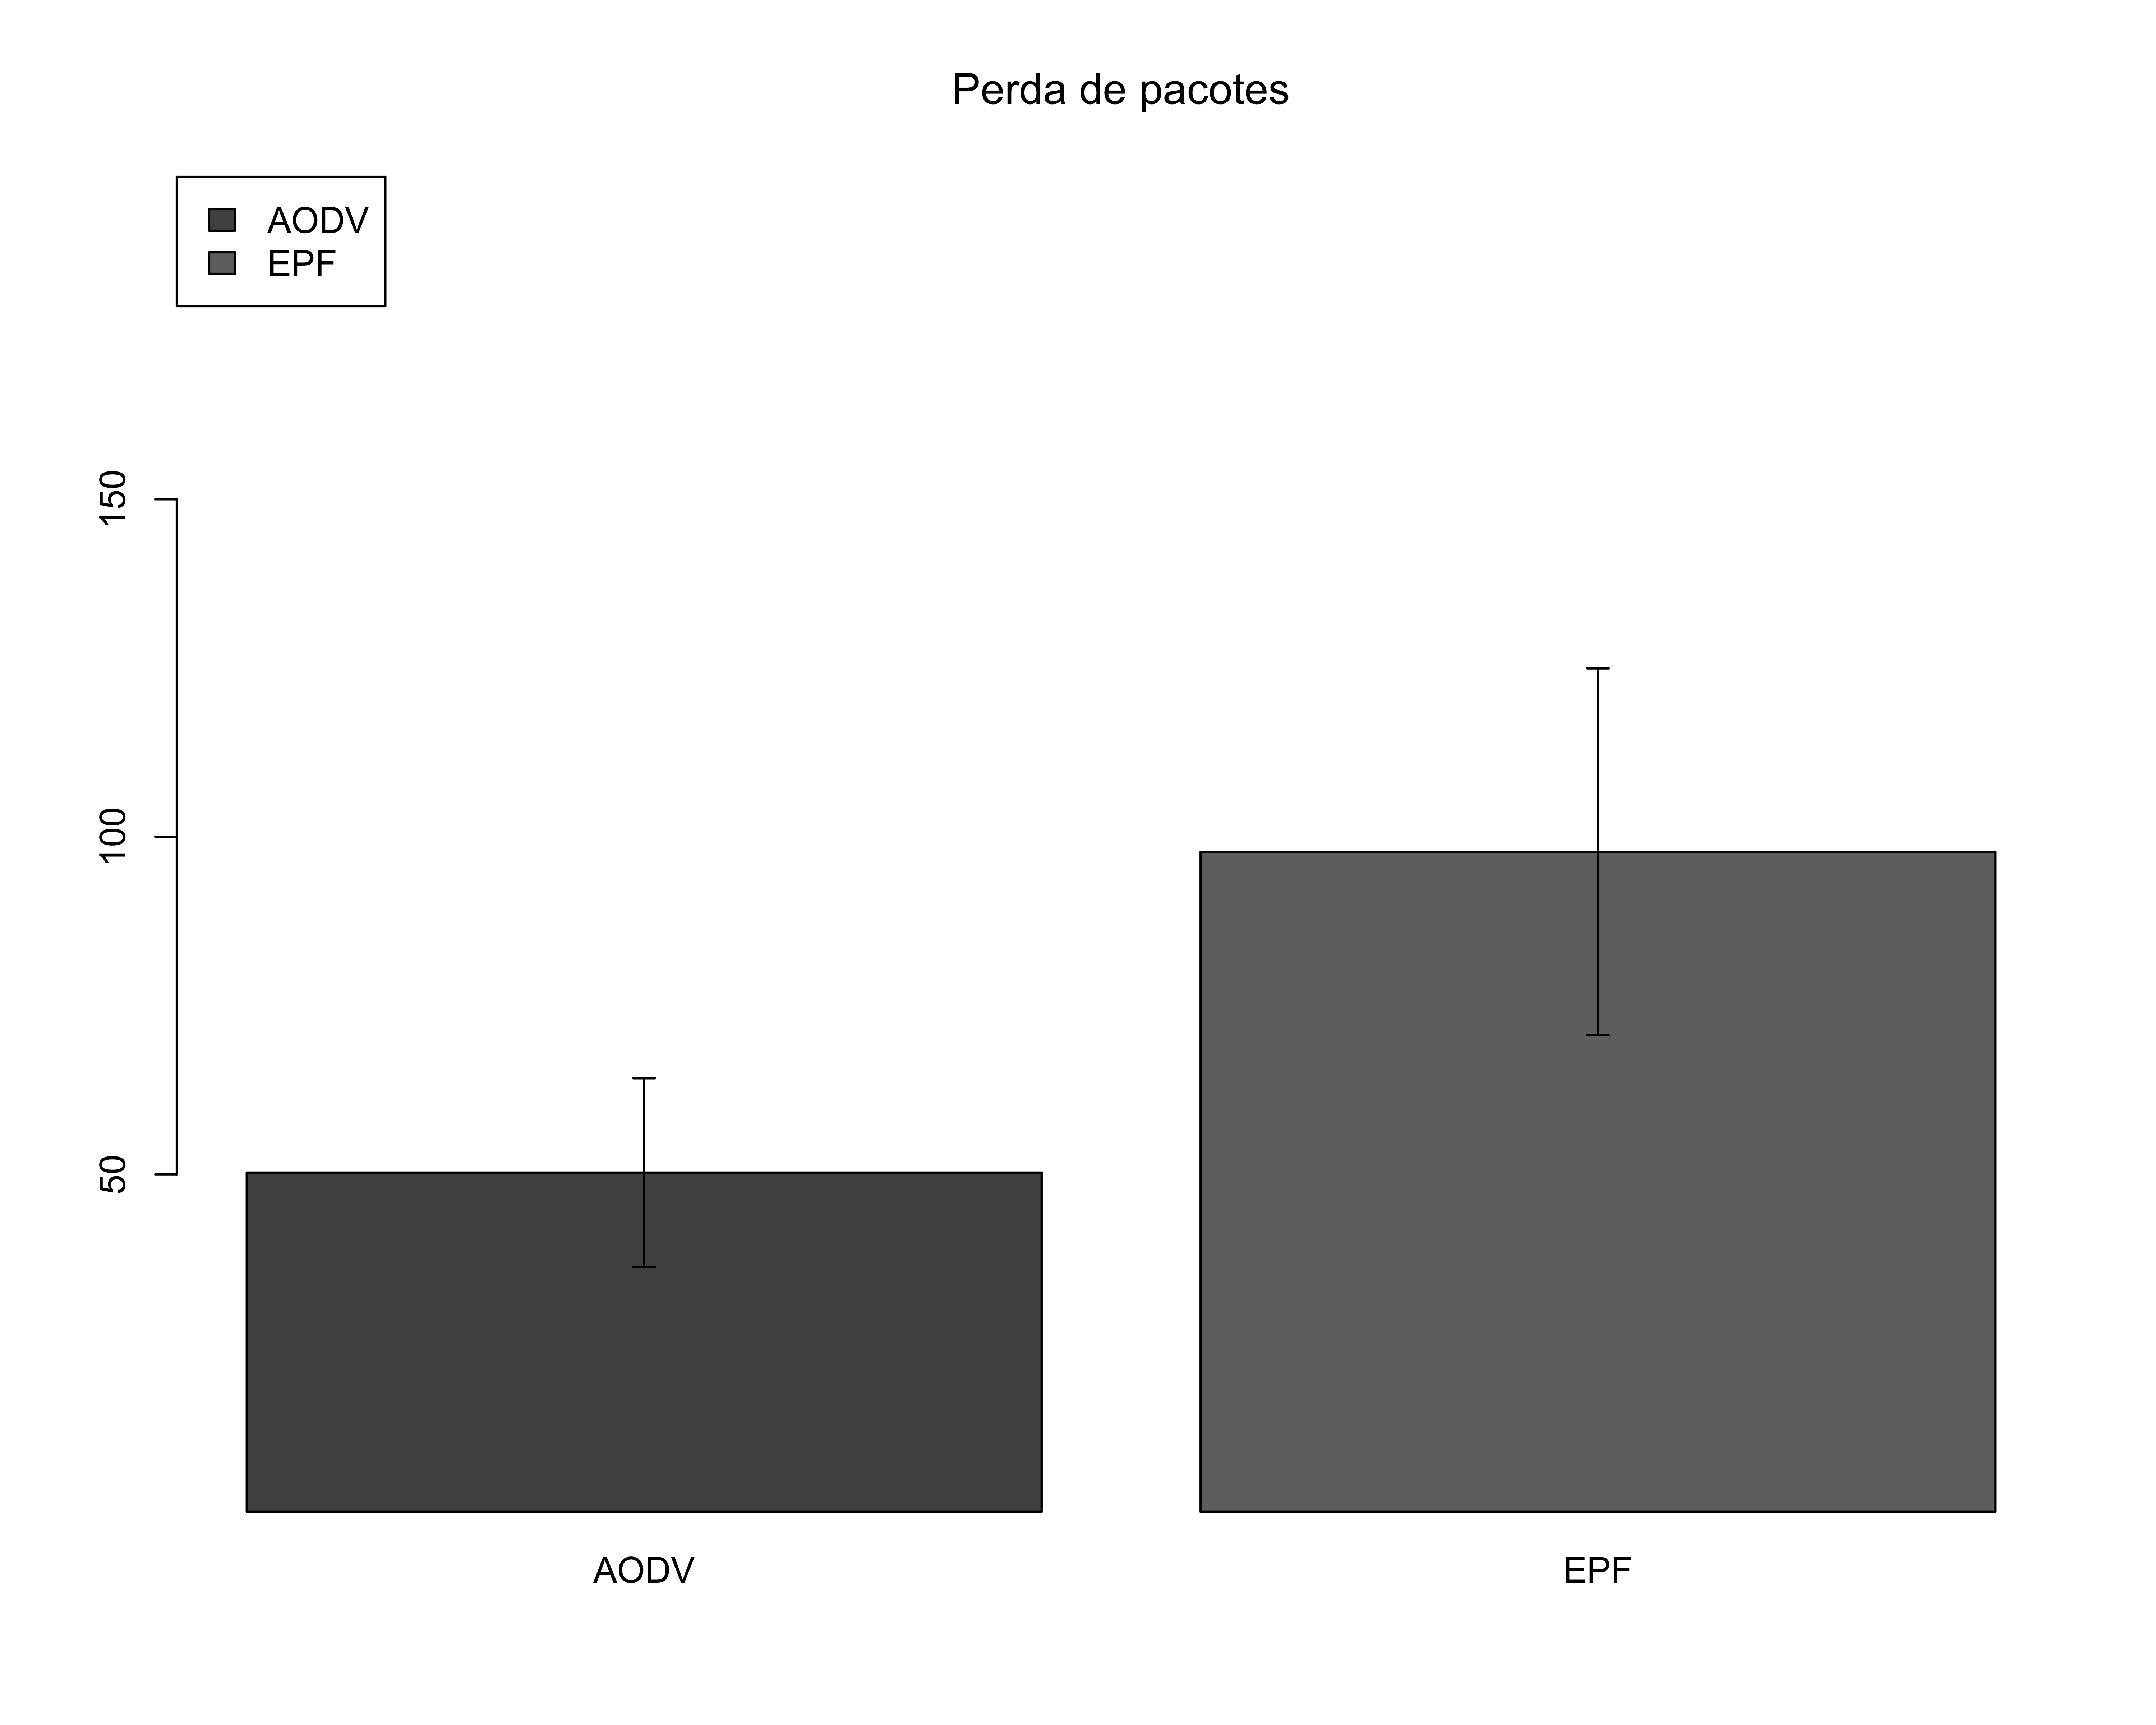
\includegraphics[height=8cm, width=0.9\textwidth]{images/drop.jpg}
\caption{Porcentagem média de mensagens perdidas.}
\label{fig:drop}
\end{figure}

\section{Resultados}\label{sec:results}

Aqui, os resultados obtidos dos testes serão mostrados e discutidos.
O primeiro resultado a ser apresentado é a coparação entre comunicação dos cenários LTE puro e LTE com D2D.
Então, comparo a quantidade de mensagens entregue ao destino, porcentagem de mensagens perdidas, tempo de enfileiramento nos \textit{buffers} e porcentagem da quantidade de mensagens que chegam foram de ordem nos dois protocolos.
Por último, os resultados da comparação da implementação com e sem \textit{trickle} para o protocolo EPF.

Como foram feitos testes com 30 e 45 dispositivos, aqui serão mostrados os resultados com 45 dispositivos pois foram considerados mais relevantes por apresentar mais informação na rede.

\subsection{Comparação LTE e LTE com D2D}\label{subsec:lte}

A Figura~\ref{fig:lte} mostra que para a configuração com D2D (duas primeiras barras de cada conjunto), a rede LTE possui muito menos carga, indicando que a introdução de D2D na rede traz benefícios.

Percebe-se que, para o cenário com D2D, a quantidade de informação na rede é muito menor em comparação com o cenário LTE.
Além disso, é importante ressaltar que, como a diferença é muito grande, a escala está é logarítmica.

\subsection{Comparação AODV e EPF}\label{subsec:aodvepf}

As Figuras~\ref{fig:entr},~\ref{fig:drop},~\ref{fig:queue} e~\ref{fig:out} mostram as comparações entre quantidade de mensagens entregues ao destino, porcentagem de mensagens perdidas, tempo de enfileiramento e porcentagem de mensagens fora de ordem, respectivamente.

Analisando a Figura~\ref{fig:entr}, podemos perceber que o protocolo EPF entrega muito menos mensagens ao destino do que o AODV.
Isso nos mostra que sua política de encaminhamento não é eficiente, ou seja, ela não faz com que as mensagens trafeguem na rede e cheguem a seu destino final.

A Figura~\ref{fig:drop} explica um pouco o motivo de o protocolo EPF entregar quase nenhuma mensagem.
Nela é possível perceber que ele perde quase todas as mensagens enviadas.
As várias trocas de mensagens para saber se um nó pode ou não encaminhar uma informação podem ser as causadoras disso.
Com muitas trocas e com os nós se movimentando, é provável que uma comunicação não exista mais no momento do encaminhamento da informação, \textit{i.e.}, os nós não estão mais em contato.
Dessa forma, a informação é perdida dentro da rede e descartada.

\begin{figure}[ht]
\centering
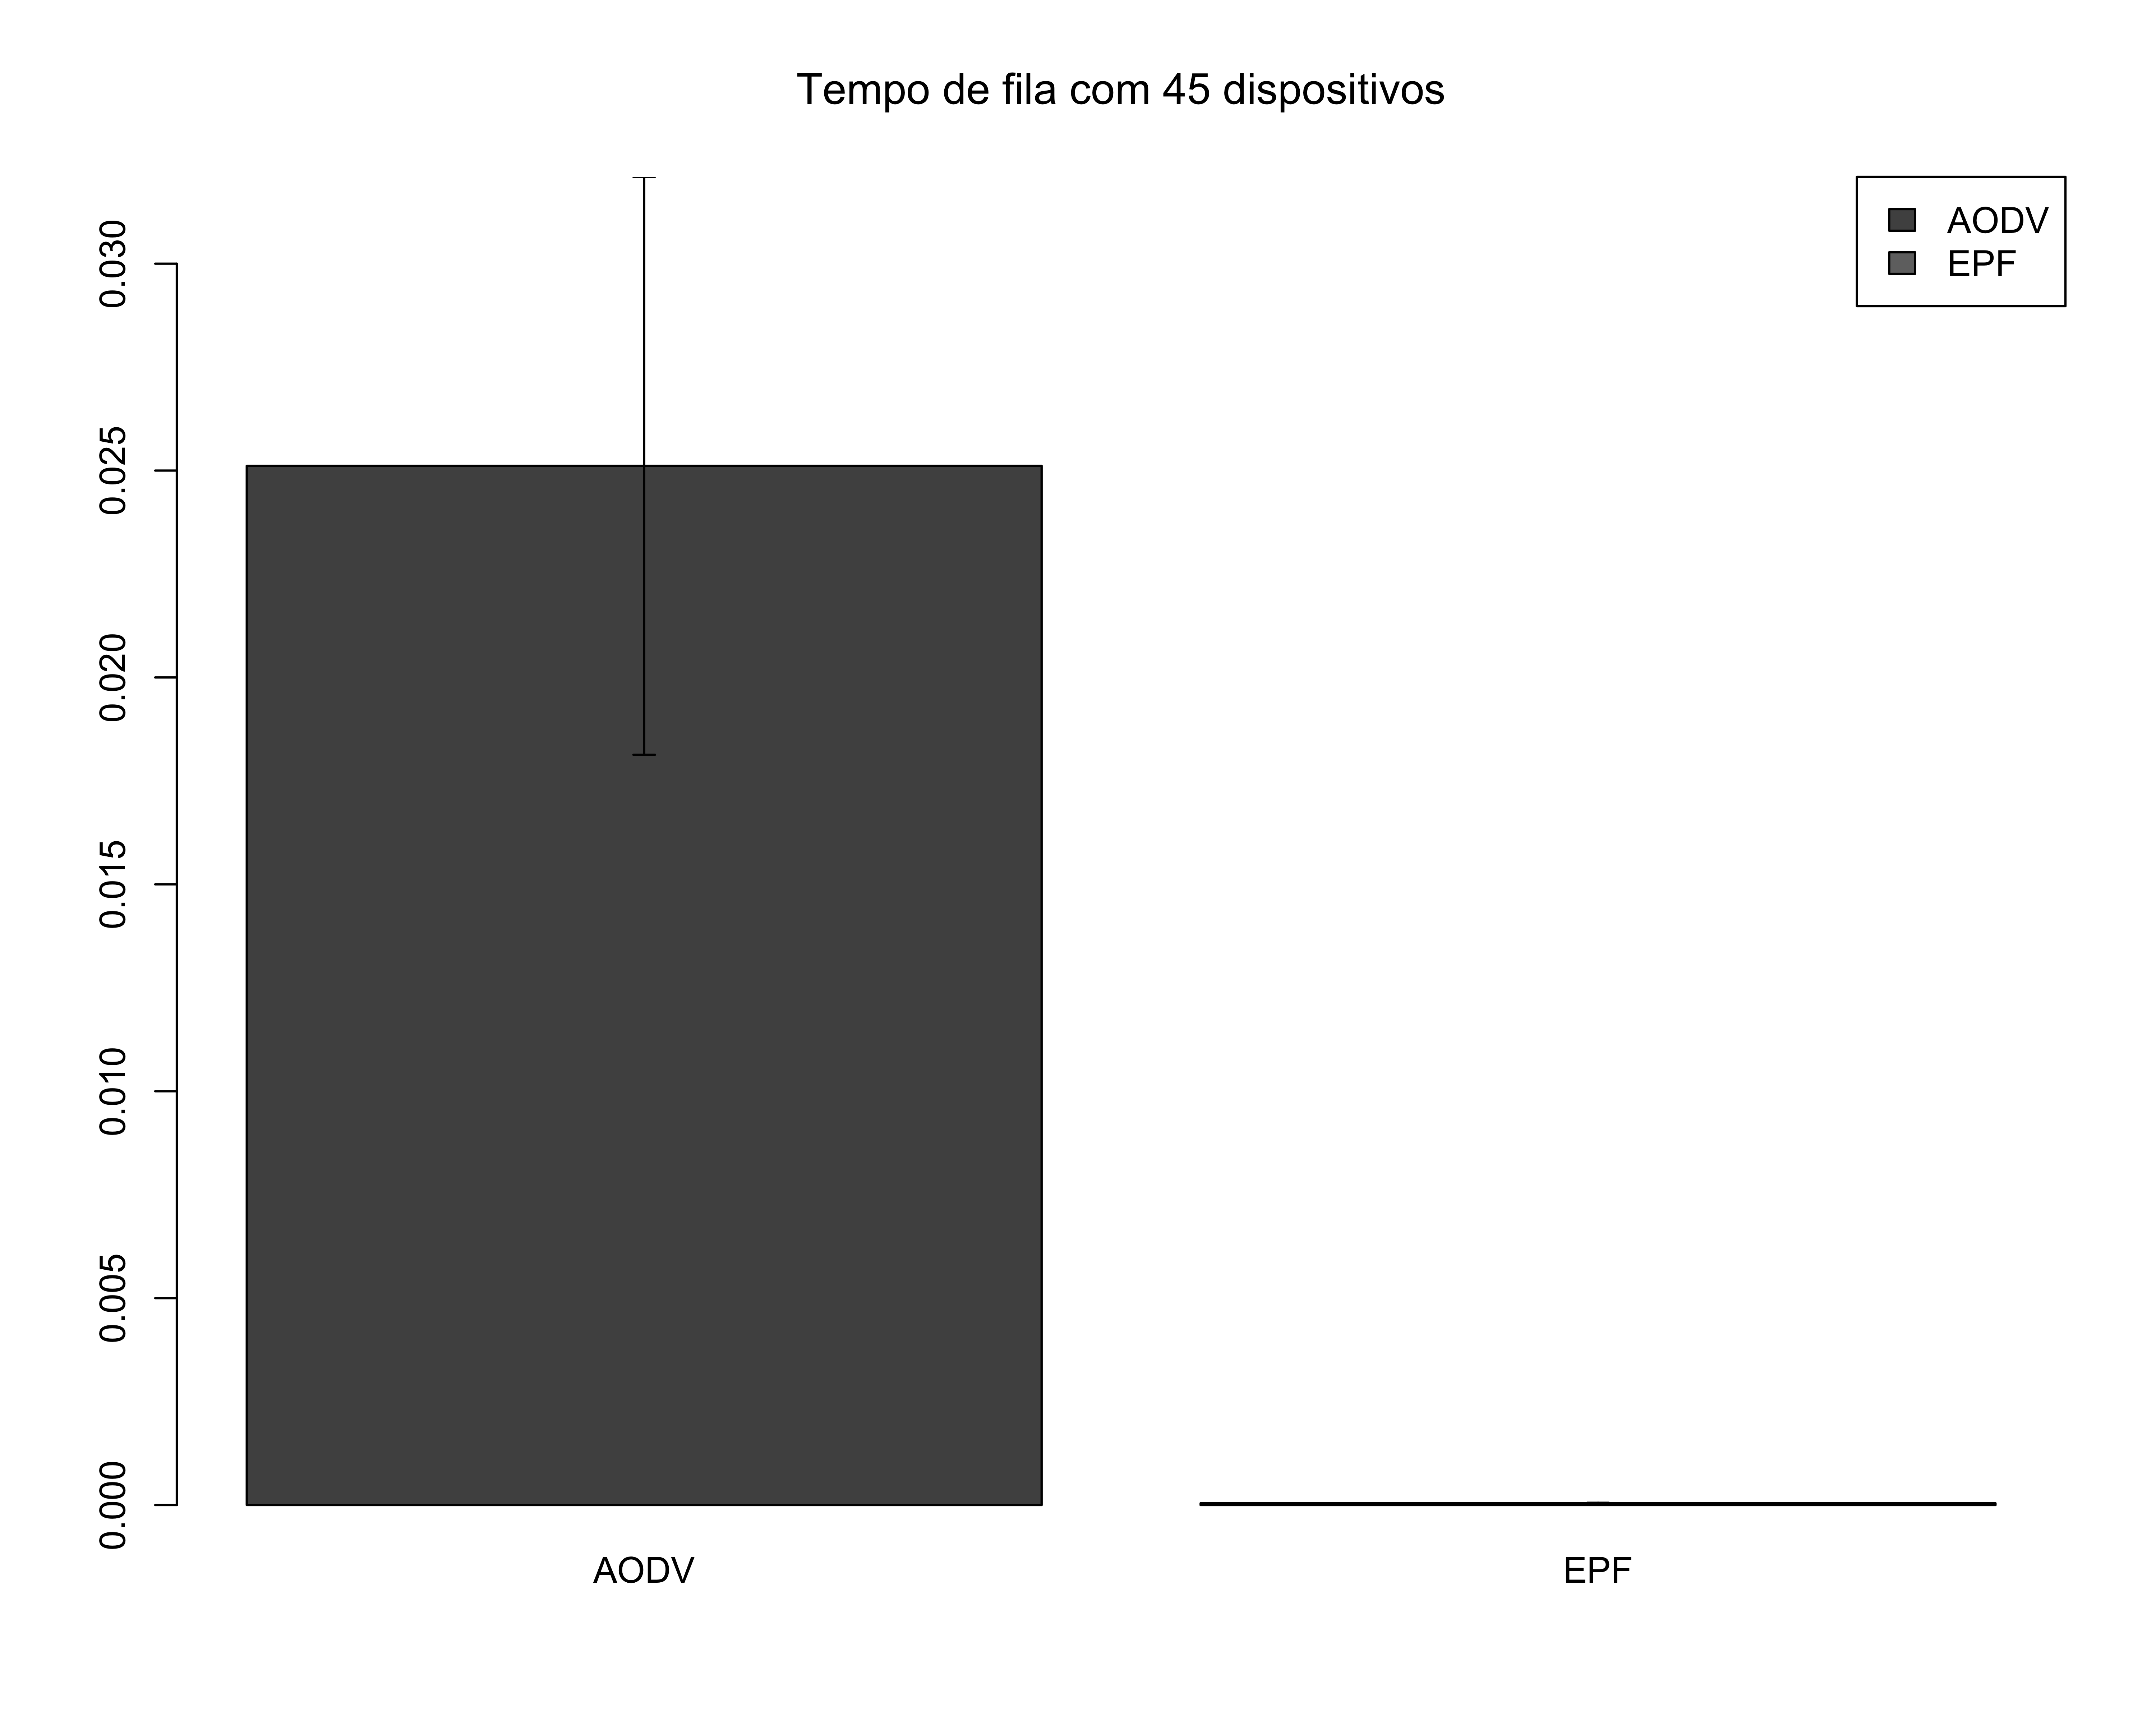
\includegraphics[height=8cm, width=0.9\textwidth]{images/queue.jpg}
\caption{Tempo médio de enfileiramento.}
\label{fig:queue}
\end{figure}

Ao analisar somente as Figuras~\ref{fig:queue} e~\ref{fig:out}, pode-se imaginar que houver resultados bons no EPF.
Porém, os números de tempo de enfileiramento e de porcentagem de mensagens fora de ordem neste protocolo são baixos devido à baixa quantidade de entrega das mensagens, como visto na Figura~\ref{fig:entr}.
Como pouquíssimas mensagens são entregues, o \textit{buffer} não se encherá, logo o tempo de enfileiramento é quase nulo.
Alé, disso, como poucas mensagens chegam, poucas chegarão fora de ordem.

\begin{figure}[ht]
\centering
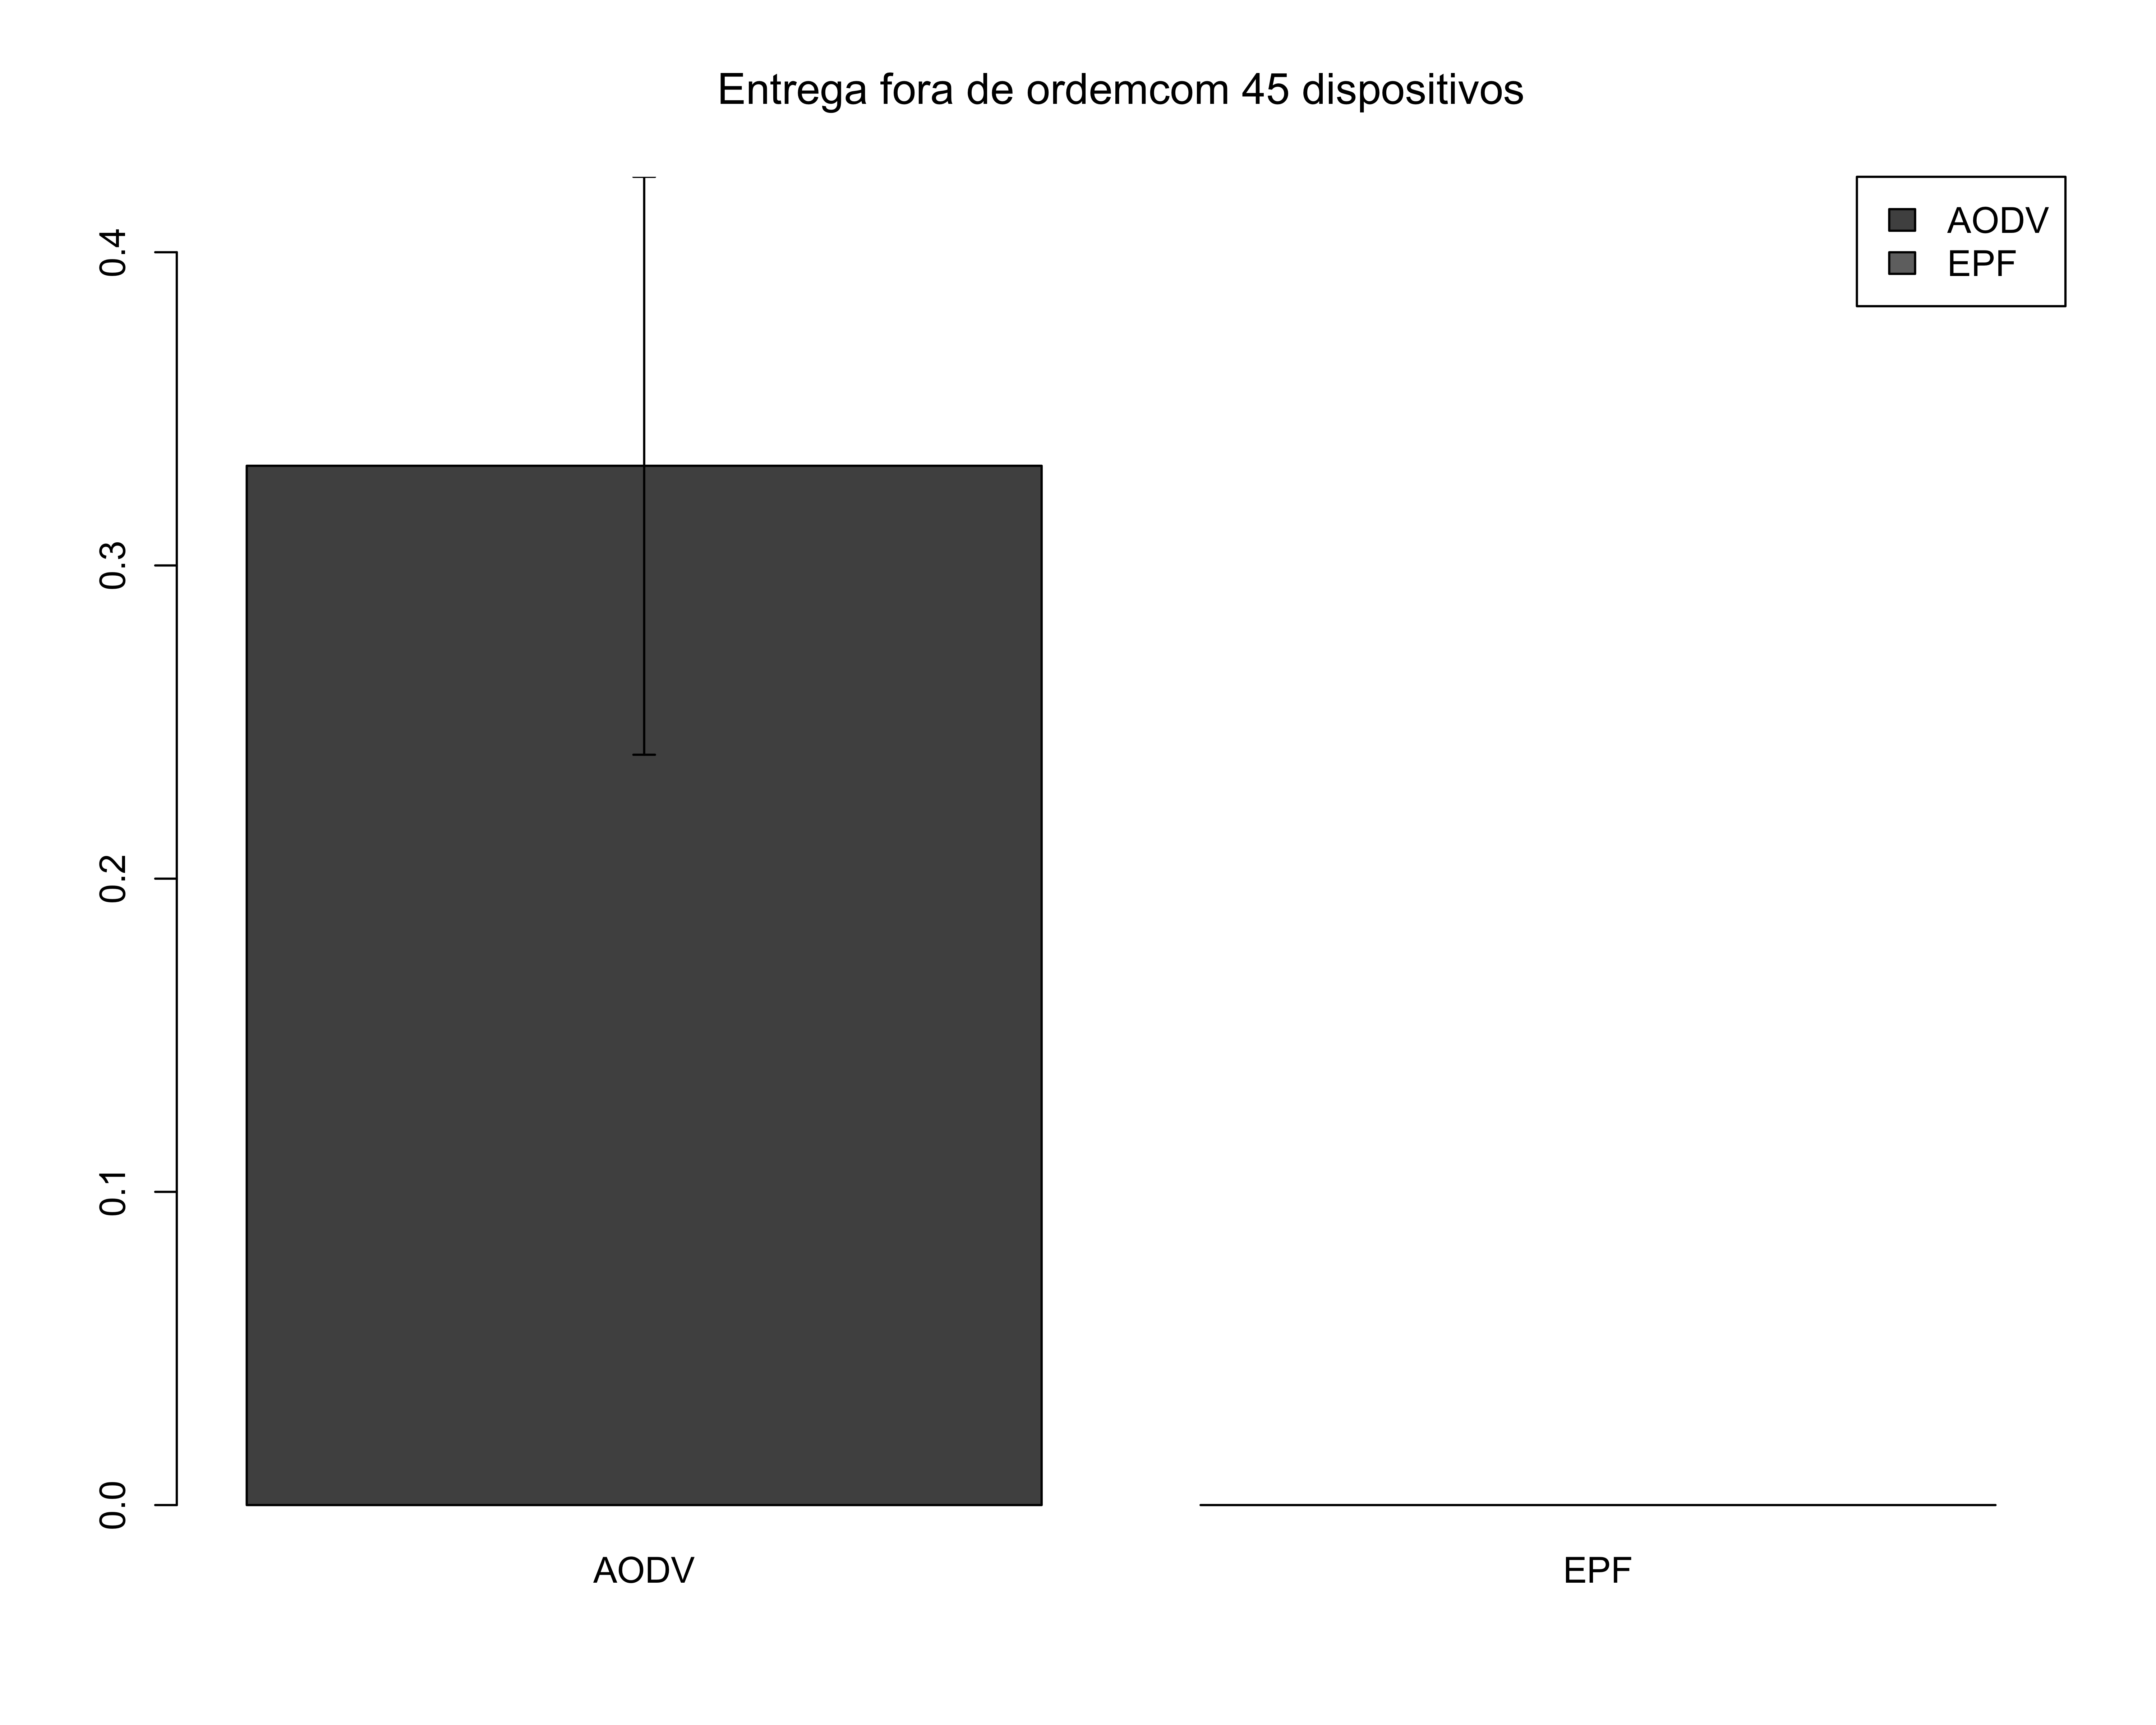
\includegraphics[height=8cm, width=0.9\textwidth]{images/out.jpg}
\caption{Porcentagem média de mensagens fora de ordem.}
\label{fig:out}
\end{figure}

\subsection{EPF com trickle}\label{subsec:epftrickle}

Como explicado Sessão~\ref{sec:trickle}, o algoritmo \textit{trickle} faz com que os protocolos enviem menos mensagens.
Com isso em vista e olhando para os resultados da subseção anterior, pode-se imaginar que o protocolo envia quase zero mensagens, e é isso que acontece.
Não considerei relevante colocar o gráfico comparando o protocolo com e sem \textit{trickle} pois a comparação é com um número muito baixo (o que não traz muita contribuição para este cenário).

\section{Considerações finais}\label{sec-consideracoes}

Com o fim deste trabalho pude perceber que a comunicação D2D traz menos carga à rede LTE, fazendo este cenário muito promissor para a implementação das redes 5G.
Além disso, vi que o protocolo proposto tem muito a melhorar, principalmente em seu principal objetivo: entregar mensagens.
Não foi possível avaliar se algoritmo \textit{trickle}, da forma como foi implementado, cumpre seu papel de limitar a quantidade de mensagens, já que mesmo sem ele, o protocolo EPF não se mostrou bom.

Para trabalhos futuros, ficam fazer mais experimentos em diferentes cenários de padrões de mobilidade e velocidade além de melhorias na forma de encaminhamento das mensagens para avaliar se o protocolo EPF da forma como foi proposto traz benefícios às redes D2D.

%%%%%%%%%%%%%%%%%%%%%%%%%%%%%%%%%%%%%%%%%%%%%%%%%%%%%%%%%%%%%%%%%%%%%%%%%%%%%%%%%%%%%%%%%%%%%%%%%%%%%%%%%%%%%%%%%%%%%%%%%%%%%%%%%%%
% Para mudar o nome da seo de referncias
%\renewcommand{\bibname}{Referncias}
%\renewcommand{\refname}{Referncias}

\bibliographystyle{unsrt}
\addcontentsline{toc}{section}{Referências}
\bibliography{references}


%%%%%%%%%%%%%%%%%%%%%%%%%%%%%%%%%%%%%%%%%%%%%%%%%%%%%%%%%%%%%%%%%%%%%%%%%%%%%%%%%%%%%%%%%%%%%%%%%%%%%%%%%%%%%%%%%%%%%%%%%%%%%%%%%%
%\appendix
%
%\pagebreak
%\section{Artigo submetido ao \textit{ACM Transactions on Interactive Intelligent Systems (TiiS)}}
%\label{sec-submissaoTIIS}

%\includegraphics{Figuras/RecSys12}


%\pagebreak
%\section{Artigo submetido ao \textit{ACM Recommender Systems 2012}}
%\label{sec-submissaoRecSys}

%\includegraphics{Figuras/RecSys12}



\end{document}

